%%%%%%%%%%%%%%%%%%% Especificación:
\begin{frame}[fragile]{Vector Clocks in Action:}{Immediate Precessors}
    \justifying
    \textbf{Un algoritmo que resuelve el problema IPT: variables locales}
    %El k-ésimo evento relevante en el proceso pk se identifica inequívocamente por el par (k,vck), donde vck es el valor de vck[k] cuando pk ha producido este evento.
    \begin{figure}
        \centering
        \begin{subfigure}[b]{\textwidth}
            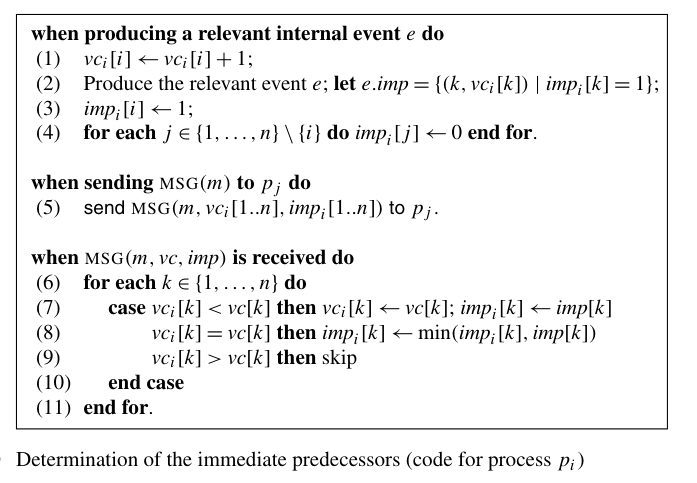
\includegraphics[scale=0.7]{Imagenes/algoIPT.png}
            \label{fig:ejemplo1}
        \end{subfigure}
    \end{figure}
\end{frame}